Based on the fundamental concepts laid out in chapter \ref{chap:literature}, chapter 3  outlines the research methodology employed to develop and evaluate an LLM-Augmented Reinforcement Learning system for automatic stock trading. It begins with section \ref{sec:overview}, an overview of the proposed solution, followed by detailed descriptions of each key component and process.

\section{Overview}
\label{sec:overview}
The proposed network operates in five key stages, beginning with data acquisition and progressing to agent training. First, \gls{OHLCV} price data and unstructured news data (headlines or summaries) are collected from financial databases, and a new dataset. Next, the news data is processed by an \gls{LLM} to extract sentiment signals, transforming raw text into quantifiable sentiment metrics. The pipeline then enters the feature engineering stage, where technical indicators derived from the \gls{OHLCV} data are combined with the \gls{LLM}-generated sentiment indicators. Finally, an environment is created with a custom reward structure to reward following the market environment, a \gls{SAC} agent is trained through iterative interaction with the environment, optimizing its policy to maximize cumulative rewards. The resulting agent autonomously executes trades by synthesizing technical signals and sentiment-driven insights, aiming to outperform sentiment-agnostic strategies. The data pipeline is demonstrated in Figure \ref{fig:pipeline}

\begin{figure}
  \centering
  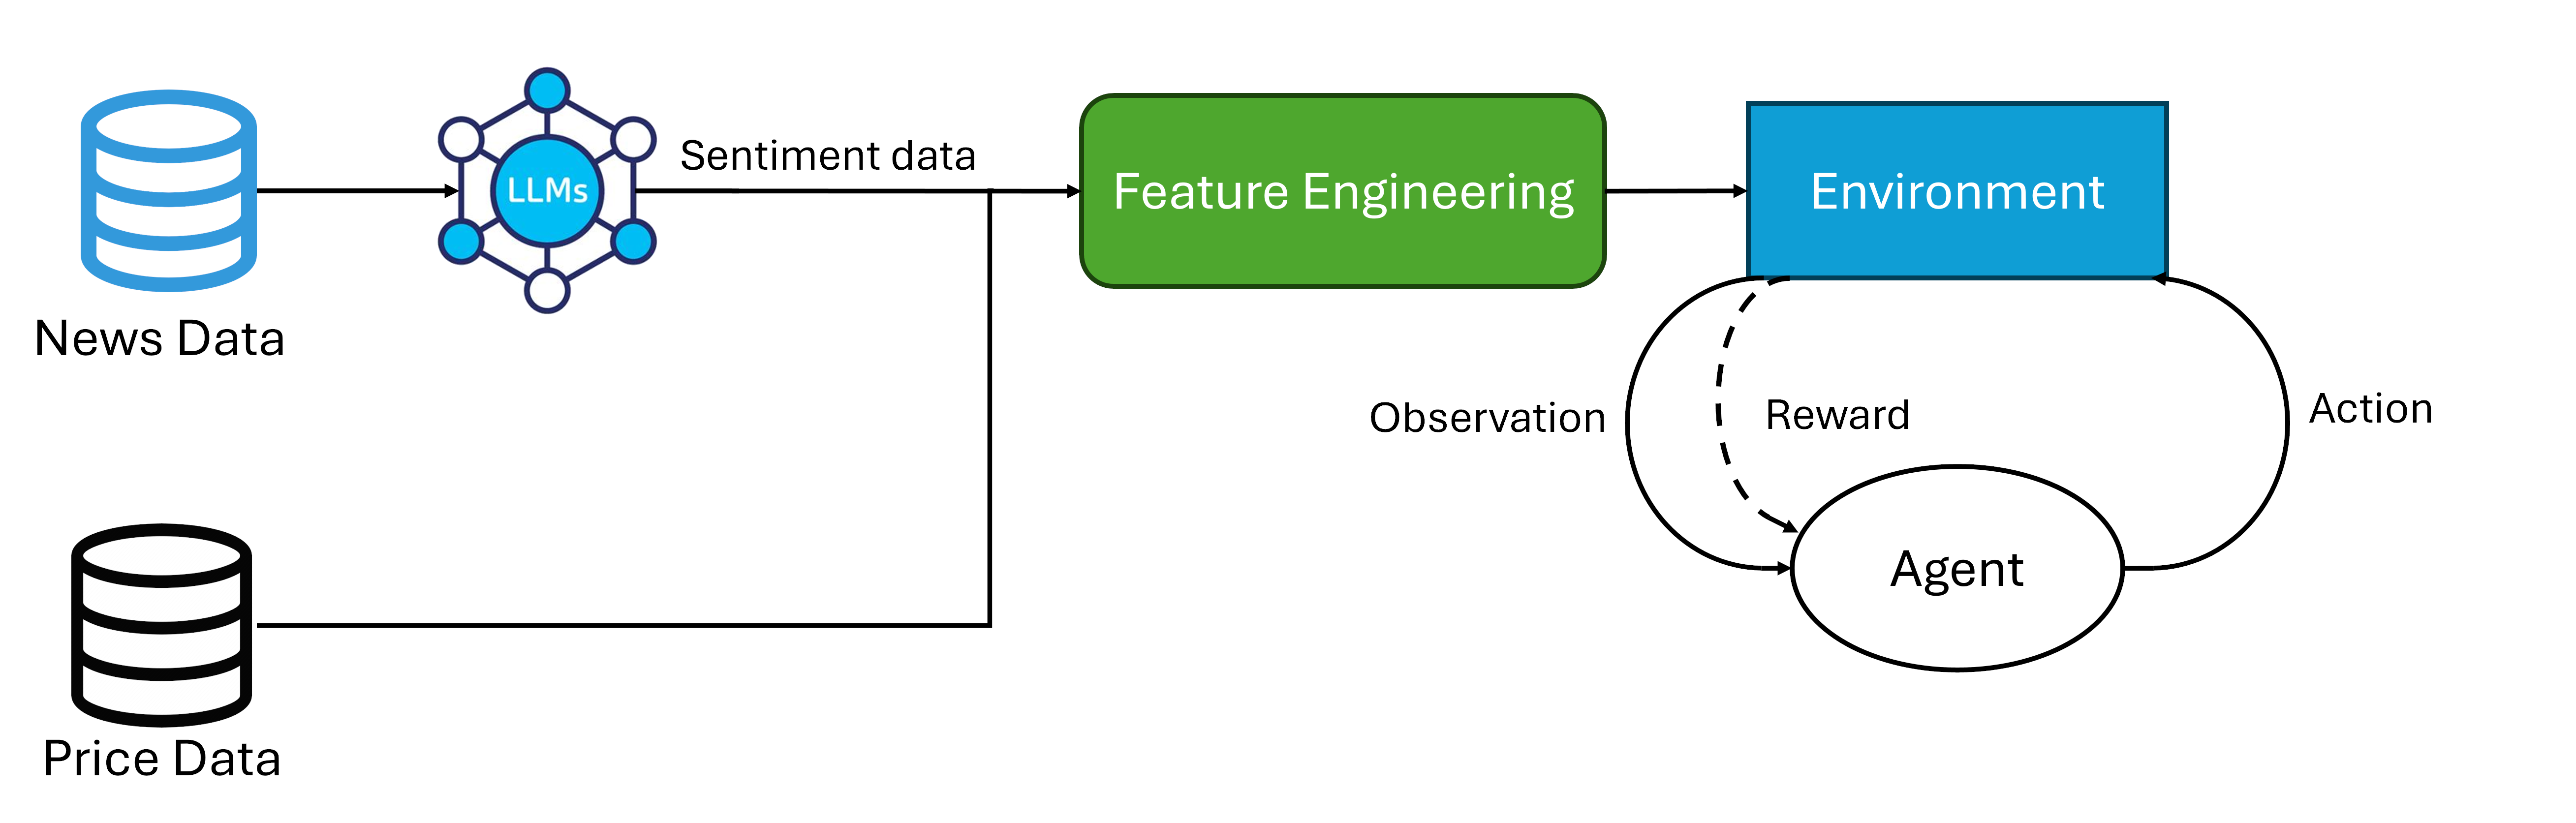
\includegraphics[width=\linewidth]{images/LLM-RL.png}
  \caption{Data pipeline of the network. News data are first sent to LLM to be processed into sentiment data before being combined with price data.}
  \label{fig:pipeline}
\end{figure}

\section{Data Acquisition}
\label{sec:data}
This section details the processes involved in gathering and preparing the necessary data, which includes historical financial market data for a defined set of stocks and a specific financial news dataset. The quality and structure of this input data are foundational to the subsequent stages of sentiment analysis, feature engineering, and \gls{RL} agent training.

\subsection{Financial Market Data}
Historical \gls{OHLCV} data for a curated list of 100 predefined stocks (stocks in the Nasdaq-100 on September 13, 2023) will be acquired. The primary source for this financial data will be the Yahoo Finance API. 

The data will cover the period from January 1, 2016, to December 28, 2023, inclusive. Data will be collected at a daily frequency. The complete dataset will be chronologically divided into training, validation, and testing sets, spanning 5 years, 1 year, and 1 year, respectively. Table \ref{tab:prices} provide a few samples of price data collected.

\begin{table}
  \centering
  \small
  \csvreader[
    tabular = {|c|c|F|F|F|F|c|},
    head to column names,
    table head = \hline Date & {Symbol} & {Open} & {High} & {Low} & {Close} & {Volume}{}\\\hline,
    late after line = \\\hline
  ]{data/sample_price.csv}{}{
    \date & \tic & \open & \high & \low & \close & \volume
  }
  \caption{Sample price data from Yahoo Finance API. These price features are common across financial application for their ability to capture important information about a stock.}
  \label{tab:prices}
\end{table}

\subsection{News Data}
For news data, this research will utilize the Financial News and Stock Price Integration Dataset (FNSPID). This dataset contains 15.7 millions financial news records for 4775 S\&P500 companies from 1999 to 2023 \cite{Dong2024}. Table \ref{tab:news} provide a new sample from the dataset. The dataset include date, news headlines, stock symbols mentioned in the content and several types of summaries. LexRank builds a similarity graph of sentences and applies a PageRank‐style algorithm to identify the most “central” sentences that best represent the document. Luhn's method scores sentences by the density and clustering of high‐frequency (non‐stop) words, favoring sentences where key terms are tightly grouped. \gls{LSA} Latent Semantic Analysis) uses singular value decomposition on the term–sentence matrix to uncover underlying thematic dimensions and then selects sentences that contribute most strongly to those principal topics. Together, these approaches offer diverse, statistically grounded summaries from which our pipeline can choose.

\begin{table}
  \centering
  \small
  \csvreader[
    respect dollar,
    head to column names,
    separator=semicolon,
    before reading=\begin{tabular}{|l|p{.7\linewidth}|}\hline,
    after reading=\end{tabular},
    late after line=\\\hline
  ]{data/sample_news.csv}{}{
      Date        & \Date \\ \hline
      Symbol      & \Symbol \\ \hline
      Headline    & \Headline \\ \hline
      Text        & \Text \\ \hline
      URL         & \URL \\ \hline
      LSA Sum     & \LSA \\ \hline
      Luhn Sum    & \Luhn \\ \hline
      TexRank Sum & \TexRank \\ \hline
      LexRank Sum & \LexRank 
  }
  \caption{Sample new data from FNSPID. The news content are processed into 4 different types of summaries making the LLM extraction process very token efficient.}
  \label{tab:news}
\end{table}

\section{Sentiment Extraction}
After news data are acquired as outline in the \ref{sec:data}, relevant news data will be processed into prompt to be sent to an \gls{LLM} model for sentiment extraction. The prompt template designed for this purpose is provided in \ref{fig:prompt}. In crafting the financial news annotation prompt, several key prompt‐engineering strategies are implemented to ensure that the model delivers precise, consistent, and machine‐readable output. The prompt begin with a clear system‐level framing, “You are an expert financial news annotator”, to establish domain context and tone. The prompt then enforces a strict JSON schema by specifying exactly two fields (sentiment\_score and news\_type) and enumerating all valid category values (with “other” as a fallback), thereby constraining responses to a controlled vocabulary and simplifying downstream parsing. A concise few‐shot example of input and output further illustrates the desired format and style, boosting the ability of the model to replicate the structure. Finally, to maintain uniformity in the input text, we define a summary selection rule for our dataset, each article is preprocessed into three possible summaries (Lexrank summary, Luhn summary, \gls{LSA} summary), and the model is instructed to inspect these in that exact order, using only the first nonempty summary it encounters. These techniques reliably guide the model to produce consistent, high‐quality JSON annotations.

\begin{figure}[!t]
  \centering
  \small
  \lstinputlisting[
    basicstyle=\ttfamily\scriptsize,
    breaklines=true,
    frame=single,
    linewidth=\linewidth
  ]{data/prompt_template.txt}
  \caption{Prompt template used to process news data into prompts. The template is designed to encourage the model to output the correct JSON format.}
  \label{fig:prompt}
\end{figure}

The model chosen for sentiment annotation is DeepSeek-V3 model \cite{DeepSeekV3}. DeepSeek-V3, developed by DeepSeek AI, is a powerful open-source Mixture-of-Experts (MoE) large language model with 671 billion parameters, of which 37 billion are active during inference. Built on a Transformer framework, it incorporates Multi-Head Latent Attention for efficient processing and DeepSeekMoE for cost-effective training.

After the sentiment scores are returned, several additional news feature are computed. First is mean sentiment:
\[\bar{s}_{i,d}  = \frac{1}{N_{i,d}} \sum_{j=1}^{N_{i,d}} s_{i,d,j}\]
where \(s_{i,d,j}\) is the sentiment score for the \(j\)-th news item about stock \(i\) on day \(d\), \(N_{i,d}\) is the total number of news items for stock \(i\) on day \(d\).

Following that, mean sentiment score of the \(k\)-th most recent news are calculated:
\[\bar{s}_{i,d}^{(k)} = \frac{1}{k} \sum_{j=1}^{k} s_{i,d,(j)}\]
where \(s_{i,d,(j)}\) is the sentiment score of the \(j\)-th most recent news item about stock \(i\) on day \(d\), and \(k\) is the number of most-recent items included in the average.

\section{Feature Engineering}

Upon successful data acquisition and sentiment extraction, the pipeline advances to the feature engineering stage. This crucial phase involves the creation of a comprehensive set of input variables, or features, that will inform the decision-making process of the \gls{RL} agent. The technical indicators are calculated from the historical \gls{OHLCV} data for each of the selected stocks. These indicators are widely used in financial analysis to identify trends, momentum, volatility, and potential overbought or oversold conditions. The following specific technical indicators will be computed: \gls{MACD}, \gls{BB}, \gls{RSI}, \gls{CCI}, and \gls{DMI}.

\subsection{Moving Average Convergence Divergence}
The \gls{MACD} is a momentum indicator that illustrates the relationship between two \gls{EMA} of a security's closing price. It is used to identify changes in trend strength, direction, momentum, and duration.

For any look-back period \(n\), define the \gls{EMA} smoothing coefficient as:
\[\alpha_n = \frac{2}{n+1}\]
The exponential moving average of the closing price \(C_t\) at time \(t\) is given recursively by:
\[\mathrm{EMA}_{n,t} = \alpha_n C_t + (1 - \alpha_n) \mathrm{EMA}_{n,t-1} , \quad \mathrm{EMA}_{n,0} := C_0\]
The standard \gls{MACD} line is the difference between a “fast” \gls{EMA} (\(n=12\)) and a “slow” \gls{EMA} (\(n=26\)):
\[\mathrm{MACD}_t = \mathrm{EMA}_{12,t} - \mathrm{EMA}_{26,t}\]
Many practitioners also compute a 9-period \gls{EMA} of the \gls{MACD} line (signal line) and plot the difference as a histogram:
\[\mathrm{Signal}_t = \mathrm{EMA}_{9}\bigl(\mathrm{MACD}\bigr)_t, \qquad \mathrm{Hist}_t = \mathrm{MACD}_t - \mathrm{Signal}_t\]

In practice, cross-overs of the \gls{MACD} line and its signal line generate buy and sell signals, while divergences between the \gls{MACD} and price can foreshadow potential trend reversals. Adjusting the \gls{EMA} periods allows traders to tune the sensitivity of the indicator to match different timeframes and volatility regimes.

\subsection{Bollinger Bands (Upper and Lower)}
The \gls{BB} are volatility indicators that measure the dispersion of price around a simple moving average, providing dynamic support and resistance levels.

Let the \(n\)-period simple moving average (SMA) of the closing price \(C_t\) be:
\[\mathrm{SMA}_{n,t} = \frac{1}{n} \sum_{i=0}^{n-1} C_{t-i}\]
Define the \(n\)-period rolling standard deviation of \(C_t\) by:
\[\sigma_{n,t} = \sqrt{\frac{1}{n} \sum_{i=0}^{n-1} (C_{t-i} - \mathrm{SMA}_{n,t})^2}\]
Then the upper and lower Bollinger Bands with multiplier \(k\) are:
\[\mathrm{BOLL\_UB}_{n,t} = \mathrm{SMA}_{n,t} + k \sigma_{n,t}, \qquad \mathrm{BOLL\_LB}_{n,t} = \mathrm{SMA}_{n,t} - k \sigma_{n,t}\]

In real market scenarios, prices touching or breaching the upper band suggest overbought conditions, while contacts with the lower band signal oversold conditions. Traders use \gls{BB} to gauge volatility expansion and contraction, identify potential reversal points, and set dynamic entry and exit levels.

\subsection{Relative Strength Index}
The \gls{RSI} is a momentum oscillator that measures the speed and change of price movements, identifying overbought or oversold conditions.

For a look‐back period \(n\), let the price change at time \(t\) be:
\[\Delta_t \;=\; C_t \;-\; C_{t-1}\]
Define the average gain and average loss over the past \(n\) periods by:
\[\mathrm{Gain}_{n,t} = \frac{1}{n} \sum_{i=1}^{n} \max(\Delta_{t-i+1},0), \quad \mathrm{Loss}_{n,t} = \frac{1}{n} \sum_{i=1}^{n} \max(-\Delta_{t-i+1},0)\]
The relative strength is:
\[\mathrm{RS}_t = \frac{\mathrm{Gain}_{n,t}}{\mathrm{Loss}_{n,t}},\]
and the RSI is then:
\[\mathrm{RSI}_t = 100 - \frac{100}{1 + \mathrm{RS}_t}\]

When applied, \gls{RSI} values above 70 suggest overbought conditions, while values below 30 suggest oversold conditions. Traders use \gls{RSI} to time entry and exit points by spotting divergences and confirming trend strength.

\subsection{Commodity Channel Index}
The \gls{CCI} is an oscillator that measures the deviation of price from its statistical mean, highlighting cyclical overbought and oversold conditions.

For a look‐back period \(n\), define the typical price at time \(t\) as
\[\mathrm{TP}_t = \frac{H_t + L_t + C_t}{3}\]
where \(H_t\), \(L_t\), and \(C_t\) are the high, low, and closing prices.  Compute the simple moving average of the typical price:
\[\mathrm{MA}_{n,t} = \frac{1}{n} \sum_{i=0}^{n-1} \mathrm{TP}_{t-i}\]
Next, define the mean deviation of the typical price:
\[\mathrm{MD}_{n,t} = \frac{1}{n} \sum_{i=0}^{n-1} |\mathrm{TP}_{t-i} - \mathrm{MA}_{n,t}\]
The CCI is then given by:
\[\mathrm{CCI}_t = \frac{\mathrm{TP}_t - \mathrm{MA}_{n,t}}{0.015 \times \mathrm{MD}_{n,t}}\]

In practice, \gls{CCI} values above \(+100\) indicate potential overbought conditions, while values below \(-100\) signal potential oversold conditions. Traders use \gls{CCI} to spot trend strength, identify entry and exit points, and confirm divergences between price action and momentum.

\subsection{Directional Movement Index}
The Directional Movement Index (DMI) is a trend‐strength indicator that compares positive and negative directional movements relative to the true range, quantifying the presence and momentum of a price trend.

For each period \(t\), compute the upward and downward price movements:
\[\mathrm{UM}_t = H_t - H_{t-1}, \quad \mathrm{DM}_t = L_{t-1} - L_t,\]
\[
\begin{aligned}
\mathrm{DM}^+_t &= 
  \begin{cases}
    \mathrm{UM}_t, & \mathrm{UM}_t > \mathrm{DM}_t \text{ and } \mathrm{UM}_t > 0,\\
    0, & \text{otherwise},
  \end{cases}
  \\
\mathrm{DM}^-_t &= 
  \begin{cases}
    \mathrm{DM}_t, & \mathrm{DM}_t > \mathrm{UM}_t \text{ and } \mathrm{DM}_t > 0,\\
    0, & \text{otherwise}
  \end{cases}
\end{aligned}
\]
Define the true range:
\[\mathrm{TR}_t = \max(H_t - L_t, |H_t - C_{t-1}|, |L_t - C_{t-1}|)\]
Over a look‐back period \(n\), form the smoothed averages:
\[\mathrm{TR}_{n,t} = \frac{1}{n} \sum_{i=0}^{n-1} \mathrm{TR}_{t-i}, \quad \mathrm{DM}^+_{n,t} = \frac{1}{n} \sum_{i=0}^{n-1}\mathrm{DM}^+_{t-i}, \quad \mathrm{DM}^-_{n,t} = \frac{1}{n} \sum_{i=0}^{n-1} \mathrm{DM}^-_{t-i}\]
Compute the directional indicators:
\[\mathrm{DI}^+_{n,t} =100 \frac{\mathrm{DM}^+_{n,t}}{\mathrm{TR}_{n,t}}, \quad \mathrm{DI}^-_{n,t} = 100 \frac{\mathrm{DM}^-_{n,t}}{\mathrm{TR}_{n,t}}.\]
The directional index (DX) measures the difference between the two:
\[\mathrm{DX}_t = 100 \frac{|\mathrm{DI}^+_{n,t} - \mathrm{DI}^-_{n,t}|}{\mathrm{DI}^+_{n,t} + \mathrm{DI}^-_{n,t}}\]
Finally, the \gls{ADX} is the \(n\)-period simple moving average of \(\mathrm{DX}\):
\[\mathrm{ADX}_t = \frac{1}{n} \sum_{i=0}^{n-1} \mathrm{DX}_{t-i}\]

Practically, rising \gls{ADX} values indicate strengthening trend momentum (regardless of direction), while falling values signal weakening trends. Traders use \gls{DMI} and \gls{ADX} to confirm trend presence, gauge its strength, and generate trade signals when directional indicators cross.

\section{Agent Training}
The trading system is modeled as a \gls{POMDP} operating on a daily time step. At each step \(t\), the agent observes a feature vector composed of the following information: \gls{OHLCV} data, technical indicators, and sentiment signals. 

To prepare each feature series for the agent, we first convert all price columns  into log returns by taking the natural logarithm of today price over yesterday. Trading volume is smoothed by applying a logarithmic transform and standardized using a rolling mean and standard deviation over a fixed window, shifted to avoid lookahead. Oscillators like \gls{MACD} and \gls{CCI} undergo the same rolling z-score standardization. \gls{BB} are summarized into a percentage metric by comparing the current price to its upper and lower bands. Short and long term moving averages are expressed as ratios of the current price to their respective averages, minus one. \gls{RSI} and \gls{ADX}, which inherently range from \(0\) to \(100\), are simply rescaled to a \(0\)–\(1\) interval. Finally, all news sentiment metrics, including mean sentiment, news counts, and longer term rolling averages, are normalized via the same rolling z-score procedure. 

At each daily time step \(t\), the agent receives a shaped reward \(R_t\) that combines the portfolio’s log return with a sentiment-based potential shaping term. Let \(\mathbf{w}_t = (w_{1,t},\dots,w_{N,t})^\top\) denote the portfolio weights at the beginning of day \(t\), and let \(P_{j,t}\) be the closing price of asset \(j\) on day \(t\). We also extract a sentiment score \(\mathrm{sent}_j(s_t)\) for each asset \(j\) at state \(s_t\). The total reward is:
\[R_t = R_t^{\mathrm{price}} + R_t^{\mathrm{sent}}\]
where the price-based component is the weighted average log return:
\[R_t^{\mathrm{price}} = \sum_{j=1}^N w_{j,t} \log \biggl(\frac{P_{j,t}}{P_{j,t-1}}\biggr)\]
and the sentiment shaping component is defined via a potential function $\Phi(s)$:
\[\Phi(s_t) = k_{\mathrm{sent}} \sum_{j=1}^N \mathrm{sent}j(s_t) \cdot \mathrm{sgn}(w{j,t} - w_{j,t-1})\]
with \(k_{\mathrm{sent}}\) a scaling hyperparameter and \(\mathrm{sgn}(\cdot)\) the sign function. The shaping reward is then:
\[R_t^{\mathrm{sent}} = \gamma,\Phi(s_{t+1}) - \Phi(s_t)\]
where \(\gamma\) is the discount factor. This construction ensures that changes in sentiment-aligned positions yield additional guidance without altering the optimal policy under reward shaping theory.

We train a \gls{SAC} agent to maximize the expected cumulative shaped reward. The policy network outputs the parameters of a Gaussian distribution over portfolio weight adjustments. Two Q-value networks estimate the soft action-value, and a temperature parameter \(\alpha\) is automatically tuned to match a target entropy, promoting exploration. Target networks for the Q-functions are updated using Polyak averaging.

In brief, this chapter has detailed how we integrate historical price data and \gls{LLM}-extracted sentiment into a unified feature set, standardize and normalize all inputs, and created an environment with sentiment-shaped reward. A \gls{SAC} agent is then trained to learn an optimal policy.
